% \documentclass[11pt,conference]{IEEEtran}
\documentclass[sigconf]{acmart}

\usepackage{bm}
\usepackage{listings}
\usepackage{tikz}
\usepackage[]{algorithm2e}
\usepackage{subcaption}
\usepackage{xcolor}

\usetikzlibrary{matrix, fit}
\usetikzlibrary{backgrounds}
\usetikzlibrary{positioning}
\usetikzlibrary{cd}

\def\BibTeX{{\rm B\kern-.05em{\sc i\kern-.025em b}\kern-.08em
    T\kern-.1667em\lower.7ex\hbox{E}\kern-.125emX}}

% a quote environment with less left indent and no right indent
\newenvironment{myquote}{\list{}{\leftmargin=12pt\rightmargin=0pt}\item[]}{\endlist}

% "tabs" for indenting Alloy statements
\def\TA{\makebox[12pt]{}}
\def\TB{\makebox[24pt]{}}
\def\TC{\makebox[36pt]{}}
\def\TD{\makebox[48pt]{}}
\def\TE{\makebox[60pt]{}}
\def\TF{\makebox[72pt]{}}

% boldface for Alloy keywords
\def\Bopen{\textbf{open} }
\def\Bas{\textbf{as} }
\def\Bsig{\textbf{sig} }
\def\Babstract{\textbf{abstract} }
\def\Bextends{\textbf{extends} }
\def\Bset{\textbf{set} }
\def\Bpred{\textbf{pred} }
\def\Bfact{\textbf{fact} }
\def\Bfun{\textbf{fun} }
\def\Bassert{\textbf{assert} }
\def\Ball{\textbf{all} }
\def\Bsome{\textbf{some} }
\def\Bone{\textbf{one} }
\def\Belse{\textbf{else} }
\def\Bin{\textbf{in} }
\def\Band{\textbf{and} }
\def\Bor{\textbf{or} }
\def\Bnot{\textbf{not} }
\def\Bno{\textbf{no} }
\def\Bimplies{$\Rightarrow$ }
\def\Biff{\textbf{iff} }
\def\Blet{\textbf{let} }
\def\Bseq{\textbf{seq} }
\def\Bint{\textbf{Int}}
\def\Buniv{\textbf{univ}}
\def\Blone{\textbf{lone} }
\def\Bcheck{\textbf{check} }
\def\Bfor{\textbf{for} }
\def\Bseq{\textbf{seq}}
\def\Bseqint{\textbf{seq} \textbf{Int}}

\begin{document}
\pagestyle{plain}
\title{SpMV Sections}
\maketitle

\section{Sparse Matrix-Vector Multiplication}

Sparse linear algebra libraries and the methods they employ are vitally important in the domain of scientific computing (TODO: why?).  Of particular interest is the sparse matrix-vector product, which solves $y = \bm{A}x$ where $\bm{A}$ is a sparse matrix and the vectors $y$ and $x$ are dense.  Because SpMV usage is often highly repetitive within, e.g., iterative solvers, performance improvements via novel algorithms and the exploitation of modern hardware are areas of ongoing research (TODO: citations).

...why is SpMV difficult? Things like array indirection, varying sparsity patterns, it's memory bound...

As modern hardware introduces higher levels of parallelism and SpMV algorithms become more complex, the likelihood of introducing subtle bugs becomes decidedly higher.  In this section we present a method for reasoning about the structural complexities and verifying the correctness of SpMV algorithms.  We first model an abstract matrix-vector multiplication and subsequently demonstrate that a CSR SpMV algorithm is a valid functional refinement.

\subsection{Abstract Matrix-Vector Multiplication}

In order to demonstrate that an SpMV algorithm is correct, we must first create a model of matrix-vector multiplication to act as the arbiter of correctness.  The result of the matrix-vector multiplication $y = \bm{A}x$ is a densely populated vector, $y$, in which each value is the dot product of a single row of the matrix $A$ with the vector $x$.  A dot product is simply a sum of products in which each product is of two values located at the same index within two vectors, as shown in ~\figurename~\ref{fig:mvm}.

\begin{figure}
\begin{subfigure}[b]{0.5\textwidth}
  \centering
  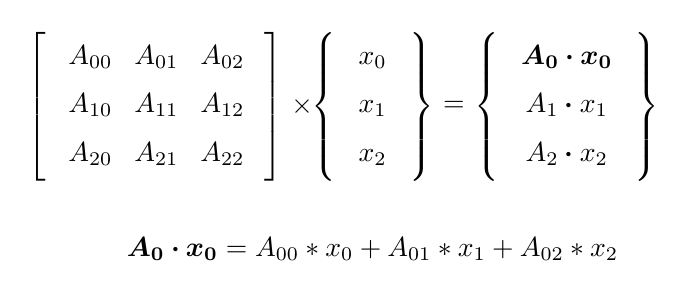
\begin{tikzpicture}

\matrix (A) [
  matrix of math nodes,
  row sep=.5ex,
  column sep=.5ex,
  left delimiter={[},right delimiter={]},
  nodes={text width=1.5em, text height=1.5ex, text depth=.5ex, align=center}
]
{
  A_{00} & A_{01} & A_{02} \\
  A_{10} & A_{11} & A_{12} \\
  A_{20} & A_{21} & A_{22} \\
};

\node (times) [right=0.75em of A] {$\times$};

\matrix (x) [
  matrix of math nodes,
  left delimiter=\{,
  right delimiter=\},
  row sep=.5ex,
  nodes={text height=1.5ex, text depth=.5ex,}, 
  right=of A
] {
  x_0\\
  x_1\\
  x_2\\
};

\node (eq) [right=1em of x] {$=$};

\matrix (b) [
  matrix of math nodes,
  left delimiter=\{,
  right delimiter=\},
  row sep=.5ex,
  nodes={text height=1.5ex, text depth=.5ex},
  right=1em of eq
] {
  \bm{A_0 \cdot x_0}\\
  A_1 \bm{\cdot} x_1\\
  A_2 \bm{\cdot} x_2\\
};

\node (A0x0) [below=1.5 em of x] {
  $\bm{A_0 \cdot x_0} = A_{00}*x_0 + A_{01}*x_1 + A_{02}*x_2$ 
};

\end{tikzpicture}
  \caption{}
  \label{fig:mvm}
\end{subfigure}
{\color{lightgray}\rule{0.4\textwidth}{0.1pt}}
\par\bigskip
\begin{subfigure}[b]{0.5\textwidth}
  \centering
  \begin{myquote}
\Bpred dotProd [row: \Bint$\rightarrow$Value, x: Matrix, b: SumProd] \\
\{\\
\TA \Ball col: row.\Buniv\ $|$\\
\TB b.values[col] = row[col]$\rightarrow$x.values[col][0]\\
\TA \Ball col: \Bint - row.\Buniv\ $|$\\
\TB \Bno b.values[col]\\
\}
\end{myquote}
  \caption{}
  \label{fig:dp}
\end{subfigure}
{\color{lightgray}\rule{0.4\textwidth}{0.1pt}}
\par\bigskip
\begin{subfigure}[b]{0.5\textwidth}
  \centering
  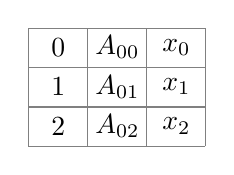
\begin{tikzpicture}
\draw[xstep=0.75cm,ystep=0.5cm,color=gray] (0,0) grid (2.25,1.5);
\matrix[matrix of math nodes,
inner sep=0pt,
anchor=south west,
nodes={inner sep=0pt,text width=.75cm,align=center,minimum height=.5cm,anchor=center}
]{
0 & A_{00} & x_0\\
1 & A_{01} & x_1\\
2 & A_{02} & x_2\\
};
\end{tikzpicture}
  \caption{}
  \label{fig:dpt}
\end{subfigure}
\caption{(\subref{fig:mvm}) a matrix-vector multiplication, (\subref{fig:dp}) the components of the first dot product in (\subref{fig:mvm}), and (\subref{fig:dpt}) the relational form of the same dot product.}
\end{figure}

Thus far, our matrix and sparse matrix models are capable of representing the structure of the matrix and vectors, as well as the values contained in $\bm{A}$ and $x$.  However, because we wish to model the \emph{structural} behavior of the algorithm, the resulting vector, $y$, cannot simply contain abstract values.  Some mechanism that allows us to determine the origin of values in the dot product is required so that we can reason about whether or not the dot product is the correct composition of values.  This is achieved using the \texttt{DotProd} signature, introduced in Section~\ref{sec:dotprod}.  Additionally, we require some mechanism for equating dot products, allowing us to determine if the solutions generated by differing algorithms are equivalent.  This is achieved using the \texttt{valEqv} predicate introduced in Section~\ref{sec:valeqv}.

\subsubsection{Dot Product Model}
\label{sec:dotprod}

Hi.
\begin{figure}
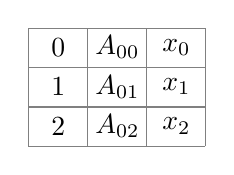
\begin{tikzpicture}
\draw[xstep=0.75cm,ystep=0.5cm,color=gray] (0,0) grid (2.25,1.5);
\matrix[matrix of math nodes,
inner sep=0pt,
anchor=south west,
nodes={inner sep=0pt,text width=.75cm,align=center,minimum height=.5cm,anchor=center}
]{
0 & A_{00} & x_0\\
1 & A_{01} & x_1\\
2 & A_{02} & x_2\\
};
\end{tikzpicture}
\end{figure}

\subsubsection{Dot Product Equivalence}
\label{sec:valeqv}

Hi.

\bibliography{sparse}

\end{document}